% Name: Smooth curve through points
% Description: The vapor pressure of water at six temperatures, joined by a smooth curve through the measured points.
% Tags: smooth curve, interpolation, data points, vapor pressure

\usepackage{pgfplots}
\pgfplotsset{compat=1.18}

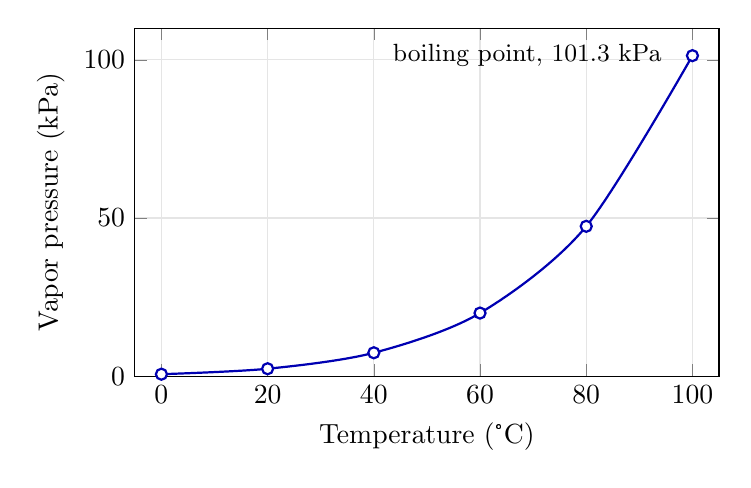
\begin{tikzpicture}
  \begin{axis}[
    width=9cm, height=6cm, xmin=-5, xmax=105, ymin=0, ymax=110,
    xlabel={Temperature (\textdegree C)}, ylabel={Vapor pressure (kPa)},
    xtick={0,20,...,100}, grid=major, grid style={gray!20},
  ]
    \addplot[smooth, thick, blue!70!black, mark=*, mark options={fill=white}] coordinates {
      (0,0.611) (20,2.339) (40,7.384) (60,19.946) (80,47.373) (100,101.325)
    };
    \node[anchor=east, font=\small] at (axis cs:96,101.325) {boiling point, 101.3 kPa};
  \end{axis}
\end{tikzpicture}
